\section{CMS} \label{section: CMS}

CMS (Compact Muon Solenoid) is one of the four detectors of the Large Hadron Collider (LHC). It is made of (starting from the center) a tracker, made of silicon sensors, that can measure the trajectory of the particles. Then, comes the electromagnetic calorimeter ECAL, which measures the energy of the electrons and the photos by stopping them completely via interactions (showers) with the environment, here PbWO$_4$. Around ECAL stands HCAL, the hadron calorimeter, which also stops the hadrons and reconstructs their energy via sensors. This is followed by a huge superconducting magnet, inducing a very strong magnetic field, that can bend the trajectory of the particles. This allows us to retrieve information in the tracker about the sign of the charge of the particle due to the possible bending of its trajectory by the magnetic field. Finally, the last layer of the detector is the muon detector.

\begin{figure}[hbt]
    \centering
    \includegraphics[width=0.7\linewidth]{Images/3.CMS/cms_160312_02.png}
    \caption{The CMS detector (cite)}
    \label{fig: CMS detector}
\end{figure}

Collisions in the detector happen every 25 ns, to retrieve the information from the collisions, CMS uses a multi-level trigger system. The CMS trigger system consists of:
\begin{itemize}
    \item Level 1 (L1) trigger: this trigger is implemented using FPGA (Field Programmable Gate Array) and ASICs (Application-Specific Integrated Circuit) and allows for a fast readout of the detector with limited granularity
    \item High Level Trigger (HLT): the events that are accepted by the L1 trigger are passed to the HLT. This trigger is implemented as software algorithms that run on large clusters of commercial processors.
\end{itemize}

\subsection{Kinematic variables}
The definitions of the observables that will be used in the following sections are reported here. Figure \ref{fig: coord syst} shows the CMS coordinate system.

\begin{figure}[hbt]
    \centering
    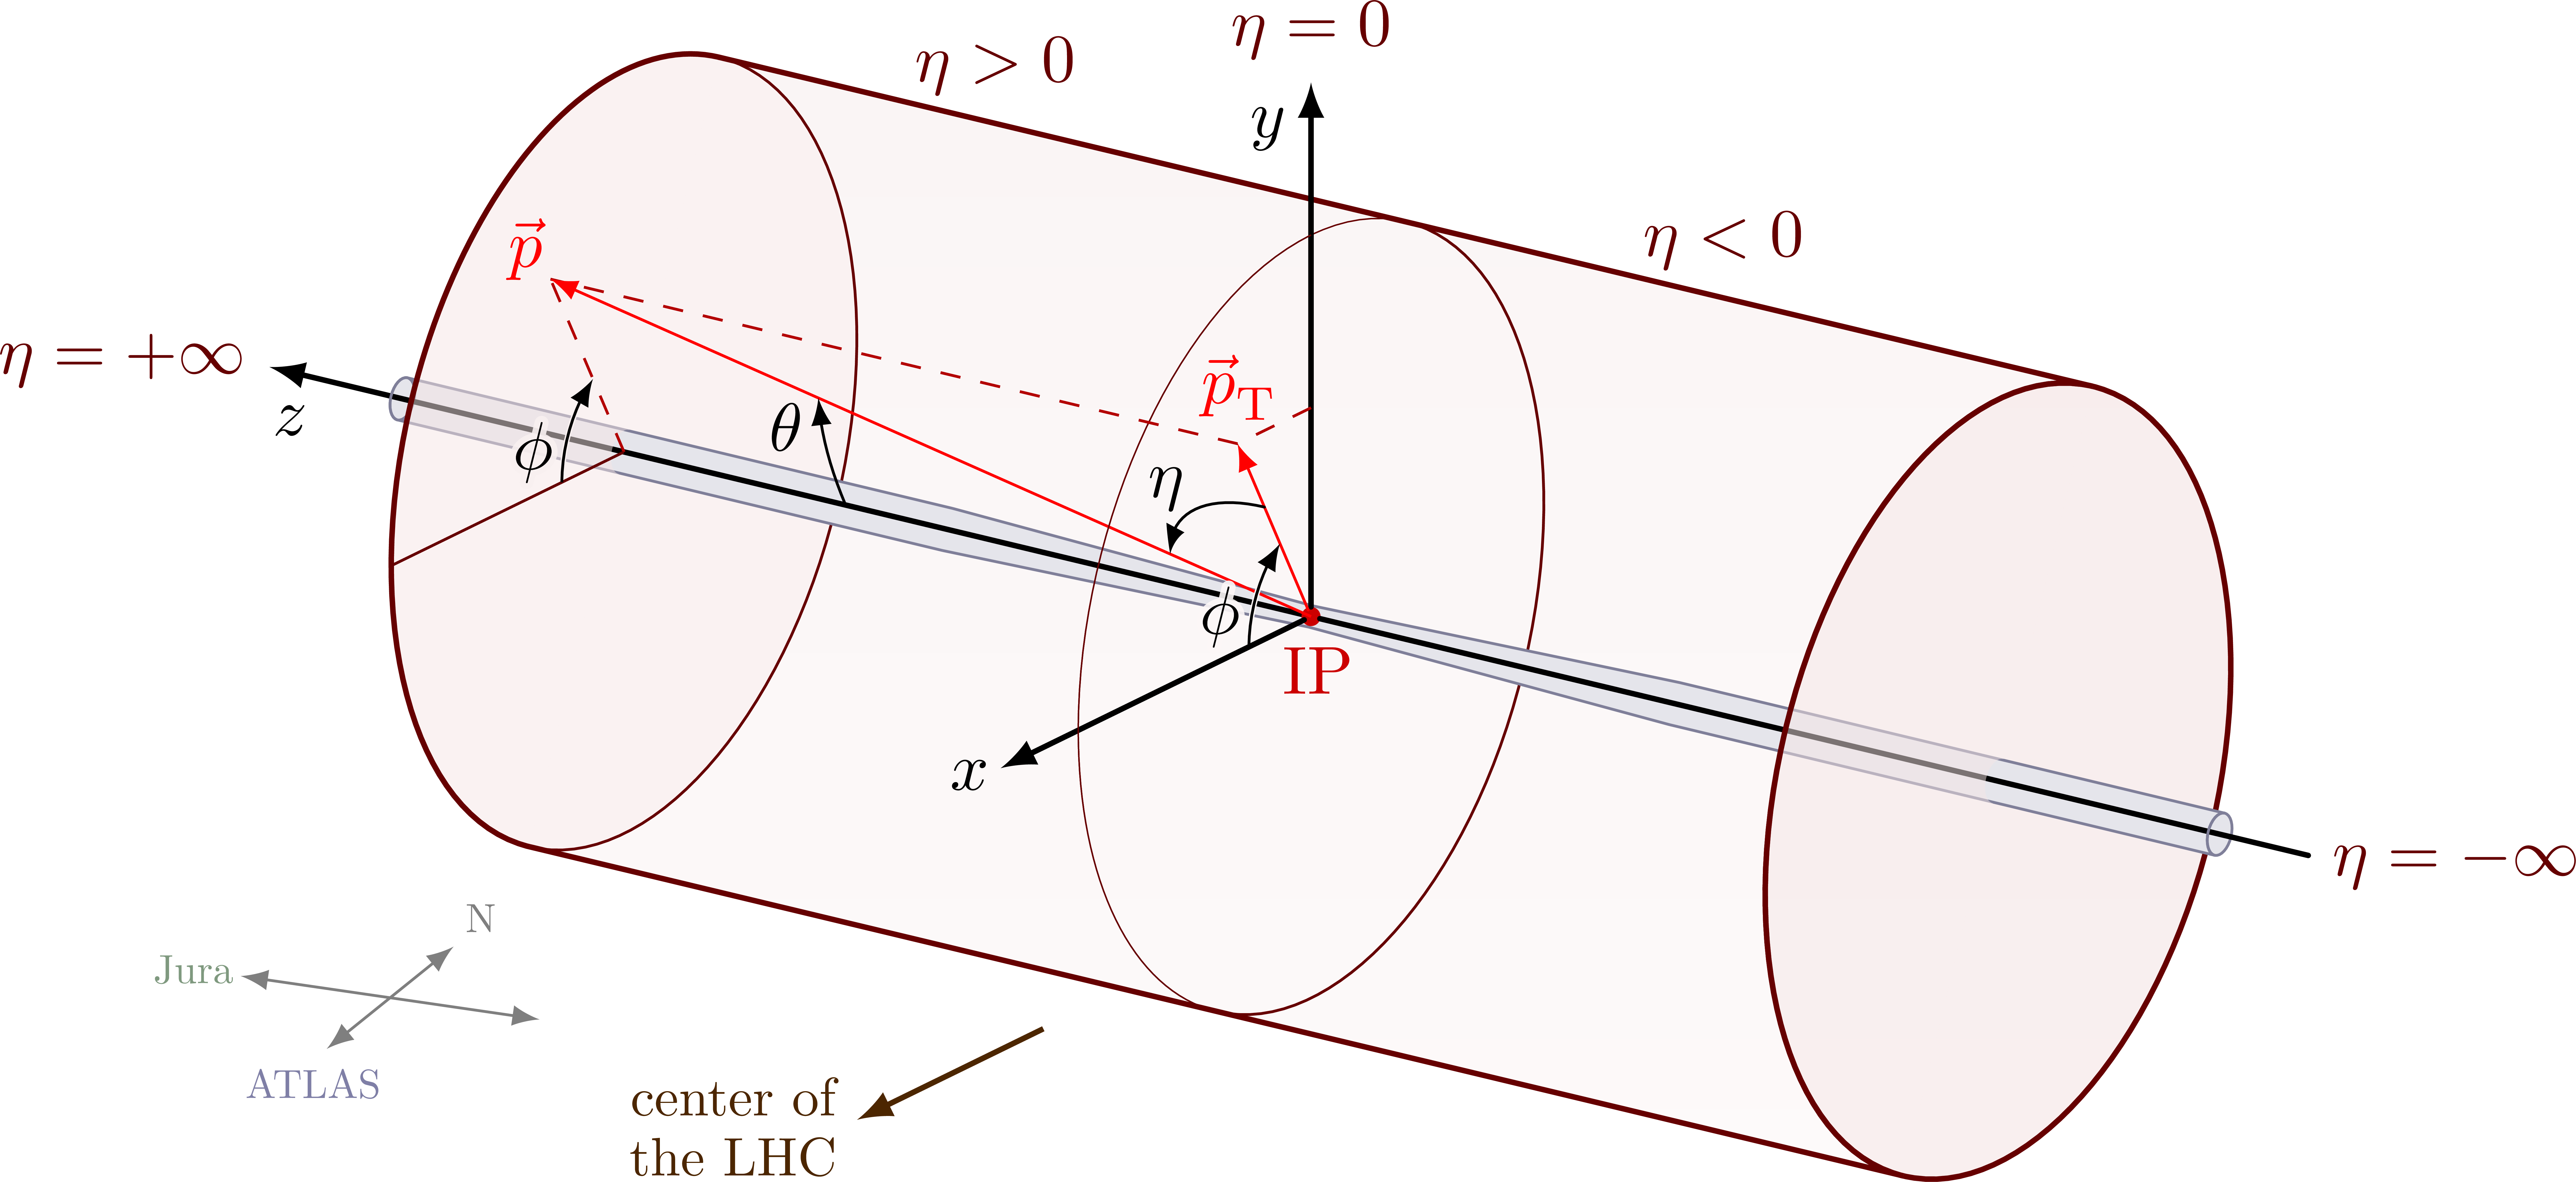
\includegraphics[width=0.7\linewidth]{Images/4.HH4b Analysis/axis3D_CMS-005.png}
    \caption{Coordinate system of the CMS detector}
    \label{fig: coord syst}
\end{figure}

\begin{itemize}
    \item Transverse momentum of the particles \pt, projection of the momentum in the transverse plane, as shown Figure \ref{fig: coord syst}
    \item \pt regressed (\pt reg), by using the ParticleNet neural network it is possible to correct the raw jet \pt to the truth-level jet energy. To do so, two components are taken into account: the \pt is adjusted to be closer to the generator-level jet \pt, and the presence of neutrinos, not reconstructed in the detector, is also taken into account.
    \item The pseudo-rapidity $\eta$, defined as:
    \begin{equation}
        \eta=-ln\bigg(\text{tan}(\frac{\theta}{2})\bigg)
    \end{equation}
    with $\theta$ being the angle between the beam axis ($z$) and the deviated particle or jet. When the deviation is low, the pseudo-rapidity either tends to $\pm \infty$ depending if it is along the beam axis or in the opposite direction (see Figure \ref{fig: coord syst}).
    \item $\Phi$ is the azimuthal angle in the $xy$ plane. Since this angle is in the transverse plane it is Lorentz invariant.
    \item $\Delta R$ is the angular distance between two objects (particles, jets). It is defined as:
    \begin{equation}
        \Delta R = \sqrt{(\Delta \eta)^2 + (\Delta \Phi)^2 }
    \end{equation}
    $\eta, \Phi$ is the metric used since $\Delta \eta$ is Lorentz invariant and so is $\Phi$.
    \item \Ht is the sum of all the \pt of the jets
    \item b-tagging is the identification (tagging) of jets containing the decay of a B hadron (b jets). The ParticleNet is used to identify the flavor of the jet, the outcome of this network is the b-tag score. The closer the score is to one, the more likely it is to be a jet originating from a b quark. We define three working points (WPs):
    \begin{itemize}
        \item Tight WP: by considering this WP there is 0.1\% of misidentification (mistagging) of the flavor of the jet, i.e. only 0.1\% of the events above this point are jets coming from a quark with a lighter flavor or a gluon but are classified as b jets.
        \item Medium WP: by considering this WP there is 1\% of misidentification of the flavour of the jet
        \item Loose WP: by considering this WP there is 10\% of misidentification of the flavor of the jet
    \end{itemize}
    \item Impact parameter $d_0$ is the distance between the daughter particle trajectory and the mother particle production point (do I add a figure?). The impact parameter in the $xy$ plane is noted $d_{xy}$ and along the z-axis $d_z$
\end{itemize}


%Maybe nno need of too much on this part

% \subsection{Tracker}
% \subsection{Electromagnetic calorimeter (ECAL)}
% \subsection{Hadronic Calorimeter (HCAL)}
% \subsection{Solenoid}
% \subsection{Muon detector}
% \subsection{Triggers}
% \subsection{Event recontsruction}
% \subsubsection{Primary Vertex}
% \subsubsection{Pile-up}
% \subsubsection{Jet reconstruction}
% \subsubsection{Missing Energy}
% \subsubsection{B-tagging} \label{Btagging} b tag algorithms are used and the fact that we use th e btag fpr the morphing to 2b to 4b
% \subsubsection{pt reg} \label{subsubsec: btag-ptreg}
% The \pt regressed is the one computed using a DNN. The main idea is that, we train a DNN with information from the reco jets and we try to retrieve the original energy if these jets. For efficiency purposes this DNNN gives out the ratio of the predicted E/ original E. To improve the analysis, we use \pt reg, which means that we multiply the \pt measured by the detector times this ratio, which allows us ti have a more precise value of thee \pt of the objects we are using.
% \subsection{Monte-Carlo}
% \subsubsection{Gen/Reco jets}

% 0.1 perccent if misidentification if the flaviur
% 1
% 10